\section{Data Pipeline}
\label{sec:data_pipeline}

We build a robust annotation pipeline that re-annotates seven open-source video sources with metric-scale camera poses, yielding a 213K-clip corpus; Fig.~\ref{fig:data_pipeline} summarizes the construction flow, and Tab.~\ref{tab:data_overview} lists the resulting data.

\begin{figure}[t]
  \centering
  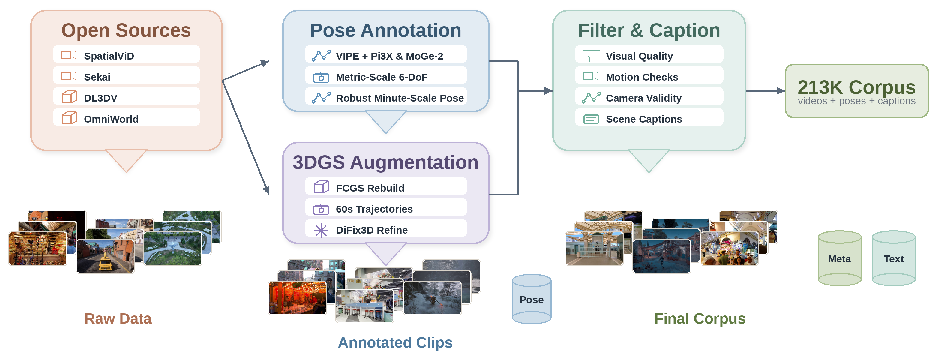
\includegraphics[width=\linewidth]{figures/data_pipeline.pdf}
  \caption{\textbf{Data construction pipeline.}
  We collect open-source video and static 3D sources, annotate metric-scale camera poses, augment DL3DV with 3DGS-rendered trajectories, and filter/caption the resulting clips into a 213K-clip training corpus.}
  \label{fig:data_pipeline}
\end{figure}

\begin{table}[h]
  \centering
  \caption{Training data overview after filtering.}
  \label{tab:data_overview}
  \footnotesize
  \begin{tabular}{llcrc}
    \toprule
    Source & Type & Duration & Clips & Pose Source \\
    \midrule
    SpatialVID-HQ~\citep{spatialvid}  & Real           & 10\,s & 158,369 & VIPE + Pi3X/MoGe-2 \\
    DL3DV~\citep{dl3dv}               & Real           & 10\,s & 5,691   & GT pose + Pi3X \\
    DL3DV~\citep{dl3dv} GS Refined    & Synthetic      & 60s & 14,881  & GT pose + Pi3X \\
    OmniWorld~\citep{omniworld}       & Synthetic      & 60s & 1,720   & VIPE + GT depth \\
    Sekai~\citep{sekai} Game          & Synthetic      & 60s & 3,560   & GT pose + Pi3X \\
    Sekai~\citep{sekai} Walking-HQ       & Real           & 60s & 9,767   & VIPE + Pi3X/MoGe-2 \\
    MiraData~\citep{miradata}         & Real & 60s & 18,987  & VIPE + Pi3X/MoGe-2 \\
    \midrule
    \textbf{Total}       &                &       & \textbf{212,975} & \\
    \bottomrule
  \end{tabular}
\end{table}


\noindent\textbf{Sources and pose annotation.}
Our annotation engine is based on VIPE~\citep{vipe}, but we found its original depth estimation unstable on long videos.
We therefore replace the depth backend with Pi3X~\citep{pi3x} and MoGe-2~\citep{moge2}: Pi3X provides long-sequence-consistent depth, while MoGe-2 provides accurate per-frame metric scale.
This yields robust metric-scale poses for long videos in the wild. We also adapt VIPE to enable per-frame intrinsic optimization for more robust internet video annotation.
For sources with provided poses, such as Sekai-Game~\citep{sekai} and DL3DV~\citep{dl3dv}, we keep the ground-truth trajectories and use Pi3X to recover metric scale.
OmniWorld~\citep{omniworld} is a special case: because it provides ground-truth depth, we use GT depth inside VIPE and use MoGe-2 for metric-scale recovery.
Engine details are in App.~\ref{sec:appendix_vipe}.

\noindent\textbf{3DGS augmentation.}
Following HY-WorldPlay~\citep{hy_worldplay}, we augment static 3D scene data with rendered camera trajectories.
DL3DV~\citep{dl3dv} contains static 3D captures rather than native one-minute videos, so we fit one FCGS~\citep{fcgs} 3D Gaussian Splatting reconstruction per scene, design diverse one-minute camera paths, and render long videos with known intrinsics and extrinsics.
We then refine the rendered videos with DiFix3D~\citep{difix3d} to reduce splatting artifacts (App.~\ref{sec:appendix_3dgs}).


\noindent\textbf{Filtering and captioning.}
We follow SANA-Video~\citep{chen2025sana} for basic visual filtering, including aesthetic quality, motion magnitude, optical-flow consistency, and scene-cut removal.
We further add camera-specific filters on field of view, focal consistency, pose smoothness, and scale variation (App.~\ref{sec:appendix_filters}).
For captioning, we follow LingBot-World~\citep{lingbot_world}: when action conditions are available, we use scene-static captions that describe objects, layout, and appearance while omitting camera actions such as ``pan left'' or ``move forward.''
This prevents text from leaking trajectory supervision and forces motion control through the pose branch.

